\documentclass{tufte-book}

\hypersetup{colorlinks}% uncomment this line if you prefer colored hyperlinks (e.g., for onscreen viewing)

%%
% Book metadata
\title{Notes on String Algorithms}
\subtitle{With Applications in Computational Biology}
\author{Kevin Gao}

%%
% If they're installed, use Bergamo and Chantilly from www.fontsite.com.
% They're clones of Bembo and Gill Sans, respectively.
%\IfFileExists{bergamo.sty}{\usepackage[osf]{bergamo}}{}% Bembo
%\IfFileExists{chantill.sty}{\usepackage{chantill}}{}% Gill Sans

%\usepackage{microtype}

%%
% Just some sample text
\usepackage{lipsum}

%%
% For nicely typeset tabular material
\usepackage{booktabs}

%%
% For graphics / images
\usepackage{graphicx}
\setkeys{Gin}{width=\linewidth,totalheight=\textheight,keepaspectratio}
\graphicspath{{figures/}}

% The fancyvrb package lets us customize the formatting of verbatim
% environments.  We use a slightly smaller font.
\usepackage{fancyvrb}
\fvset{fontsize=\normalsize}

%%
% Prints argument within hanging parentheses (i.e., parentheses that take
% up no horizontal space).  Useful in tabular environments.
\newcommand{\hangp}[1]{\makebox[0pt][r]{(}#1\makebox[0pt][l]{)}}

%%
% Prints an asterisk that takes up no horizontal space.
% Useful in tabular environments.
\newcommand{\hangstar}{\makebox[0pt][l]{*}}

%%
% Prints a trailing space in a smart way.
\usepackage{xspace}

%%
% For typesetting pseudocode
\usepackage{clrscode3e}

%%
% For typesetting math
\usepackage{amsmath}
\usepackage{amssymb}
\usepackage{amsthm}

\setcounter{tocdepth}{0}
\setcounter{secnumdepth}{0}
%%
% Theorem environments
\newtheorem{theorem}{Theorem}[chapter]
\newtheorem{lemma}[theorem]{Lemma}
\newtheorem{claim}[theorem]{Claim}
\newtheorem{corollary}[theorem]{Corollary}
\newtheorem{definition}[theorem]{Definition}
\newtheorem{remark}[theorem]{Remark}
\newtheorem{example}[theorem]{Example}

%%
% Some shortcuts for Tufte's book titles.  The lowercase commands will
% produce the initials of the book title in italics.  The all-caps commands
% will print out the full title of the book in italics.
\newcommand{\vdqi}{\textit{VDQI}\xspace}
\newcommand{\ei}{\textit{EI}\xspace}
\newcommand{\ve}{\textit{VE}\xspace}
\newcommand{\be}{\textit{BE}\xspace}
\newcommand{\VDQI}{\textit{The Visual Display of Quantitative Information}\xspace}
\newcommand{\EI}{\textit{Envisioning Information}\xspace}
\newcommand{\VE}{\textit{Visual Explanations}\xspace}
\newcommand{\BE}{\textit{Beautiful Evidence}\xspace}

\newcommand{\TL}{Tufte-\LaTeX\xspace}

% Prints the month name (e.g., January) and the year (e.g., 2008)
\newcommand{\monthyear}{%
  \ifcase\month\or January\or February\or March\or April\or May\or June\or
  July\or August\or September\or October\or November\or
  December\fi\space\number\year
}


% Prints an epigraph and speaker in sans serif, all-caps type.
\newcommand{\openepigraph}[2]{%
  %\sffamily\fontsize{14}{16}\selectfont
  \begin{fullwidth}
  \sffamily\large
  \begin{doublespace}
  \noindent\allcaps{#1}\\% epigraph
  \noindent\allcaps{#2}% author
  \end{doublespace}
  \end{fullwidth}
}

% Inserts a blank page
\newcommand{\blankpage}{\newpage\hbox{}\thispagestyle{empty}\newpage}

\usepackage{units}

% Typesets the font size, leading, and measure in the form of 10/12x26 pc.
\newcommand{\measure}[3]{#1/#2$\times$\unit[#3]{pc}}

% Macros for typesetting the documentation
\newcommand{\hlred}[1]{\textcolor{Maroon}{#1}}% prints in red
\newcommand{\hangleft}[1]{\makebox[0pt][r]{#1}}
\newcommand{\hairsp}{\hspace{1pt}}% hair space
\newcommand{\hquad}{\hskip0.5em\relax}% half quad space
\newcommand{\TODO}{\textcolor{red}{\bf TODO!}\xspace}
\newcommand{\na}{\quad--}% used in tables for N/A cells
\providecommand{\XeLaTeX}{X\lower.5ex\hbox{\kern-0.15em\reflectbox{E}}\kern-0.1em\LaTeX}
\newcommand{\tXeLaTeX}{\XeLaTeX\index{XeLaTeX@\protect\XeLaTeX}}
% \index{\texttt{\textbackslash xyz}@\hangleft{\texttt{\textbackslash}}\texttt{xyz}}
\newcommand{\tuftebs}{\symbol{'134}}% a backslash in tt type in OT1/T1
\newcommand{\doccmdnoindex}[2][]{\texttt{\tuftebs#2}}% command name -- adds backslash automatically (and doesn't add cmd to the index)
\newcommand{\doccmddef}[2][]{%
  \hlred{\texttt{\tuftebs#2}}\label{cmd:#2}%
  \ifthenelse{\isempty{#1}}%
    {% add the command to the index
      \index{#2 command@\protect\hangleft{\texttt{\tuftebs}}\texttt{#2}}% command name
    }%
    {% add the command and package to the index
      \index{#2 command@\protect\hangleft{\texttt{\tuftebs}}\texttt{#2} (\texttt{#1} package)}% command name
      \index{#1 package@\texttt{#1} package}\index{packages!#1@\texttt{#1}}% package name
    }%
}% command name -- adds backslash automatically
\newcommand{\doccmd}[2][]{%
  \texttt{\tuftebs#2}%
  \ifthenelse{\isempty{#1}}%
    {% add the command to the index
      \index{#2 command@\protect\hangleft{\texttt{\tuftebs}}\texttt{#2}}% command name
    }%
    {% add the command and package to the index
      \index{#2 command@\protect\hangleft{\texttt{\tuftebs}}\texttt{#2} (\texttt{#1} package)}% command name
      \index{#1 package@\texttt{#1} package}\index{packages!#1@\texttt{#1}}% package name
    }%
}% command name -- adds backslash automatically
\newcommand{\docopt}[1]{\ensuremath{\langle}\textrm{\textit{#1}}\ensuremath{\rangle}}% optional command argument
\newcommand{\docarg}[1]{\textrm{\textit{#1}}}% (required) command argument
\newenvironment{docspec}{\begin{quotation}\ttfamily\parskip0pt\parindent0pt\ignorespaces}{\end{quotation}}% command specification environment
\newcommand{\docenv}[1]{\texttt{#1}\index{#1 environment@\texttt{#1} environment}\index{environments!#1@\texttt{#1}}}% environment name
\newcommand{\docenvdef}[1]{\hlred{\texttt{#1}}\label{env:#1}\index{#1 environment@\texttt{#1} environment}\index{environments!#1@\texttt{#1}}}% environment name
\newcommand{\docpkg}[1]{\texttt{#1}\index{#1 package@\texttt{#1} package}\index{packages!#1@\texttt{#1}}}% package name
\newcommand{\doccls}[1]{\texttt{#1}}% document class name
\newcommand{\docclsopt}[1]{\texttt{#1}\index{#1 class option@\texttt{#1} class option}\index{class options!#1@\texttt{#1}}}% document class option name
\newcommand{\docclsoptdef}[1]{\hlred{\texttt{#1}}\label{clsopt:#1}\index{#1 class option@\texttt{#1} class option}\index{class options!#1@\texttt{#1}}}% document class option name defined
\newcommand{\docmsg}[2]{\bigskip\begin{fullwidth}\noindent\ttfamily#1\end{fullwidth}\medskip\par\noindent#2}
\newcommand{\docfilehook}[2]{\texttt{#1}\index{file hooks!#2}\index{#1@\texttt{#1}}}
\newcommand{\doccounter}[1]{\texttt{#1}\index{#1 counter@\texttt{#1} counter}}

% Generates the index
\usepackage{makeidx}
\makeindex


\titlecontents{part}
    [0pt]
    {\addvspace{0.25\baselineskip}}
    {{Part~\thecontentslabel}}
    {{Part~\thecontentslabel}}
    {}
    [\vspace*{0.5\baselineskip}]

\titlecontents{chapter}
    [4em]
    {}
    {\contentslabel{2em}\textit}
    {\hspace{0em}\textit}
    {\qquad\thecontentspage}
    [\vspace*{0.5\baselineskip}]

\begin{document}

% Front matter
\frontmatter

% r.1 blank page

% v.2 epigraphs

% r.3 full title page
\maketitle


% v.4 copyright page
\newpage
\begin{fullwidth}
~\vfill
\thispagestyle{empty}
\setlength{\parindent}{0pt}
\setlength{\parskip}{\baselineskip}
Copyright \copyright\ \the\year\ \thanklessauthor

\par\smallcaps{terra-incognita.dev}

\par Licensed under the Apache License, Version 2.0 (the ``License''); you may not
use this file except in compliance with the License. You may obtain a copy
of the License at \url{http://www.apache.org/licenses/LICENSE-2.0}. Unless
required by applicable law or agreed to in writing, software distributed
under the License is distributed on an \smallcaps{``AS IS'' BASIS, WITHOUT
WARRANTIES OR CONDITIONS OF ANY KIND}, either express or implied. See the
License for the specific language governing permissions and limitations
under the License.


\end{fullwidth}

% r.5 contents
\tableofcontents

% r.7 dedication
\cleardoublepage
~\vfill

{\noindent\fontsize{18}{22}\selectfont\itshape
\nohyphenation
These notes are primarily based on the book \textbf{Algorithms on Strings, Trees, and Sequences} by \textbf{Dan Gusfield}.

\hfill

\noindent Thanks Professor Gusfield for his great book.}

\vfill
\vfill


% r.9 introduction
\cleardoublepage


%%
% Start the main matter (normal chapters)
\mainmatter

\part{Exact Matching}

\chapter{Naive Exact Matching}
(Gusfield Section 1.1)

\newthought{Terminology Confusion}. Before starting the discussion of string matching algorithms, we should note the difference between a \textit{\textbf{substring}} and a \textit{\textbf{subsequence}}. Given a string S, characters in a substring of S must occur contiguously in S; whereas characters in a subse- quence may be interspersed gaps (or indels, as we call them in biology) and/or characters not in the original string.

\section{Exact String Mathching Problem}

Given a text string $T$ and pattern $P$, the goal of the exact string matching problem is to find all occurrences of $P$ in $T$.

\section{The ``Na\"ive'' Algorithm} \index{naive exact matching algorithm}

\begin{codebox}
    \Procname{$\proc{Naive-Match}(P,T)$}
    \li $\id{matches} = [\;]$
    \li \For $i=1$ \To $|T|-|P|+1$ \Do
        \li $\id{match} = \const{true}$
        \li \For $j = 1$ \To $|P|$ \Do
            \li \If $T[i+j] \neq P[j]$ \Then
                \li $\id{match} = \const{false}$
                \li \textbf{break}
            \End
        \li \If $\id{match}$ \Then
            \li $\id{matches}.\proc{Append}(i)$ 
        \End
    \End
    \li \Return $\id{matches}$ 
\end{codebox}

\begin{marginfigure}
    \caption{Naive exact matching with $P=abxyabxa$ and $T=xabxyabxyabxz$.}
    \begin{alignat*}{7}
        T:\; &x&&a&&b&&x&&y&&abxyabxz \\
        P:\; &a&&b&&x&&y&&a&&bxa \\
        & && a&&b&&x&&y&&abxa \\
        & && && a&&b&&x&&yabxa \\
        & && && && a&&b&&xyabxa \\
        & && && && && a &&bxyabxa \\
        & && && && && && abxyabxa \\
    \end{alignat*}
    \label{fig:naive-matching}
\end{marginfigure}

The na\"ive exact matching algorithm aligns the left end of $P$ with the left end of $T$ and compares the characters of $P$ and $T$ left to right until a mismatch is found, or until it reaches the end of $P$, in which case we report the position of $P$. Then, $P$ is shifted to the right by one place. We repeat this procedure until the right end of $P$ passes the right end of $T$.

\section{Runtime of the Naive Algorithm}

Let $n = |P|$ and $m = |T|$. The worst-case comparisons made by the naive algorithm is $\Theta(nm)$. We have the lower bound $\Omega(nm)$ when
$P$ and $T$ contains the same repeated characters (e.g. $P = aaa$, $T = aaaaaaaaa$), in which case the algorithm makes $n(m-n+1) \in \Omega(nm)$ comparisons.

\chapter{Z Algorithm}
(Gusfield Chapter 1)

\section{Speeding Up the Naive Algorithm}

The naive exact matching algorithm is stupid. It always shifts $P$ by only one even if it knows for sure that the next shift will not yield a match. This gives us some ideas on how to improve the algorithm. If we can shift $P$ by more than one character, but never shift so far as to miss the next occurrence of $P$ in $T$, we can improve the runtime of the naive algorithm.

Doing this, however, requires us to have some prior knowledge of the pattern $P$ or the text $T$.

\section{Foundamental Preprocessing}

A fundemental preprocessing is a generalized way to process the pattern $P$ to gain knowledge of the pattern, independent of any particular algorithm.

\begin{definition}
    Given a string $S$ and a position $i>1$, let $Z_i(S)$ be the length of the longest substring of $S$ that starts at $i$ and matches a prefix of $S$.

    In other words, $Z_i(S)$ is the length of the longest prefix of $S[i\ldots |S|]$ that matches a prefix of $S$.
\end{definition}

\begin{definition}[Z-box] \index{Z-box}
    For any position $i > 1$ where $Z_i$ is greater than 0, the \textbf{Z-box} at $i$ is the interval starting at $i$ and ending at $i+Z_i-1$.
\end{definition}

\begin{marginfigure}
    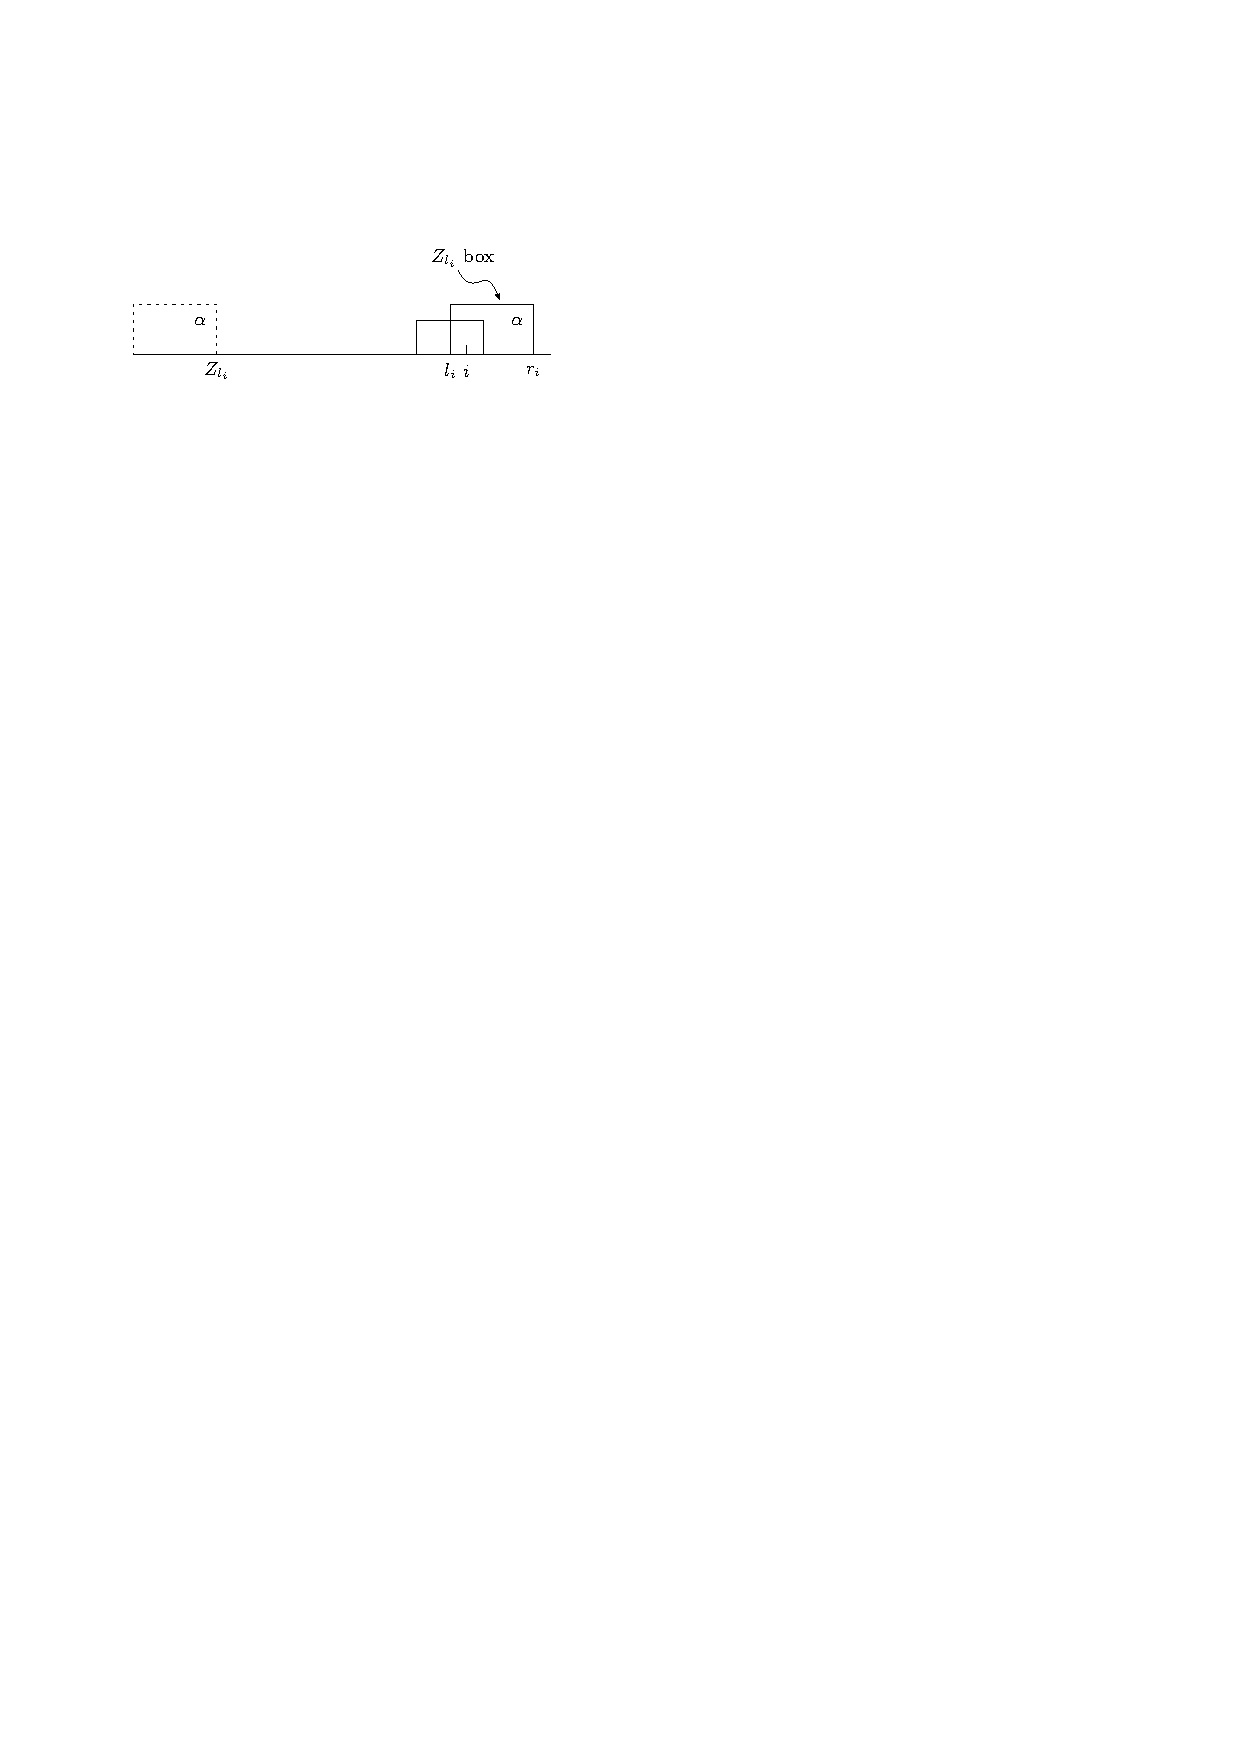
\includegraphics[width=\linewidth]{z/z-box.pdf}
    \caption{Relations between $i$, $l_i$, $r_i$ and the Z-box at $l_i$.}
    \label{fig:z-box}
\end{marginfigure}

\begin{definition}
    For every $i > 1$, $r_i$ is the right endpoint of the Z-box that begins at or befor position $i$ (i.e. the closest Z-box to the left). More formally, $r_i$ is the largest value of $j + Z_j - 1$ over all $1 < j \leq i$ such that $Z_j > 0$.
\end{definition}

\index{fundamental preprocessing}
The linear-time computation of the $Z_i$ values for all $i \in \{1,\ldots,|S|\}$ from the string $S$ is called the \textit{\textbf{fundamental preprocessing}} task.

\section{The Z Algorithm} \index{Z algorithm}

The \textit{\textbf{Z algorithm}} is an algorithm for computing the fundamental preprocessing. The Z algorithm is similar to a dynamic programming algorithm in the sense that it uses memoized information to speed up the computation and reduce the number of comparison needed. Namely, assume there exists $j < i$ such that $j + Z[j] - 1 > i$, then we can use $Z[i-j+1]$ to infer $Z[i]$.

\begin{figure}[htbp]
    \centering
    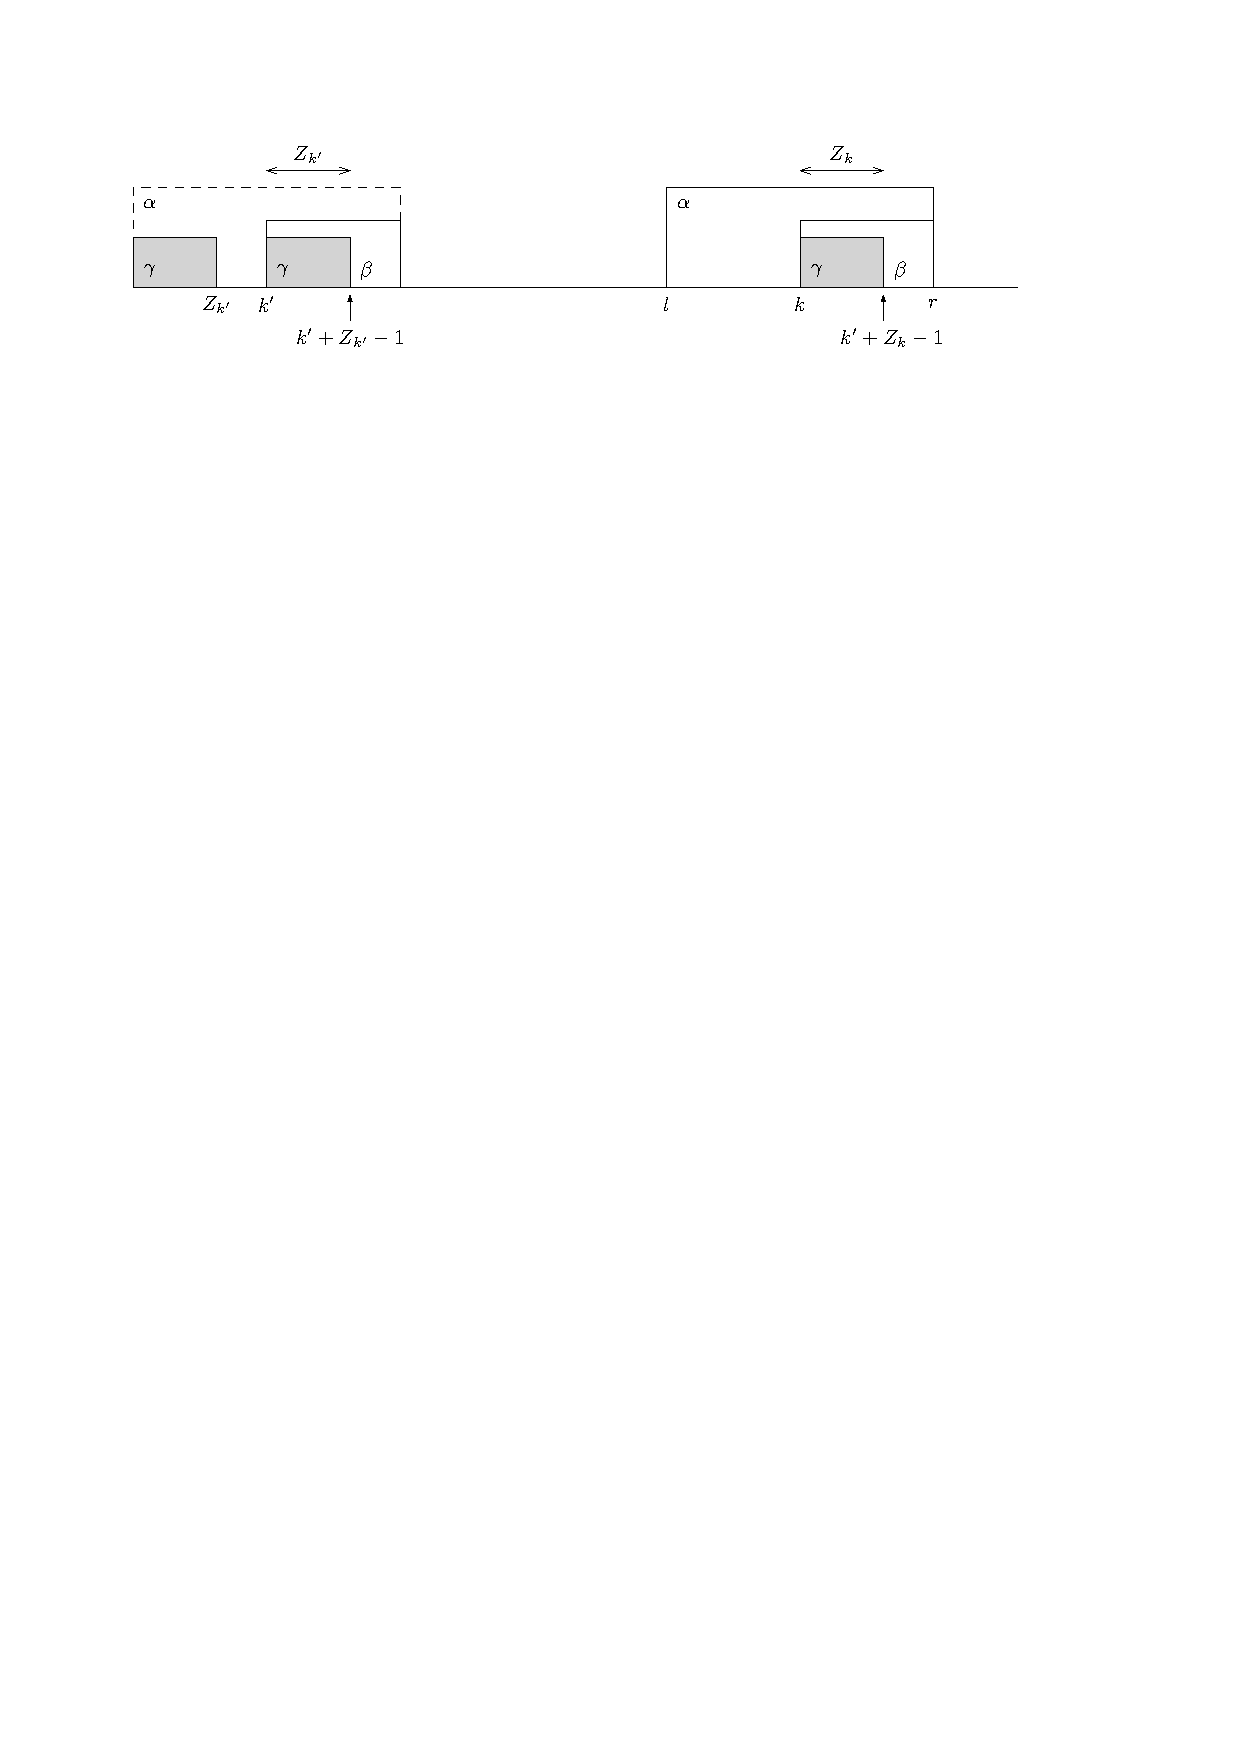
\includegraphics[width=\linewidth]{z/z-process-case2a.pdf}
    \caption{Case 2a: The longest string starting at $k'$ that matches a prefix of $S$ is shorter than $|\beta| = r-k+1$. In this case, $Z_k = Z_{k'}$.}
    \label{fig:z-process-case2a}
\end{figure}

\begin{figure}[htbp]
    \centering
    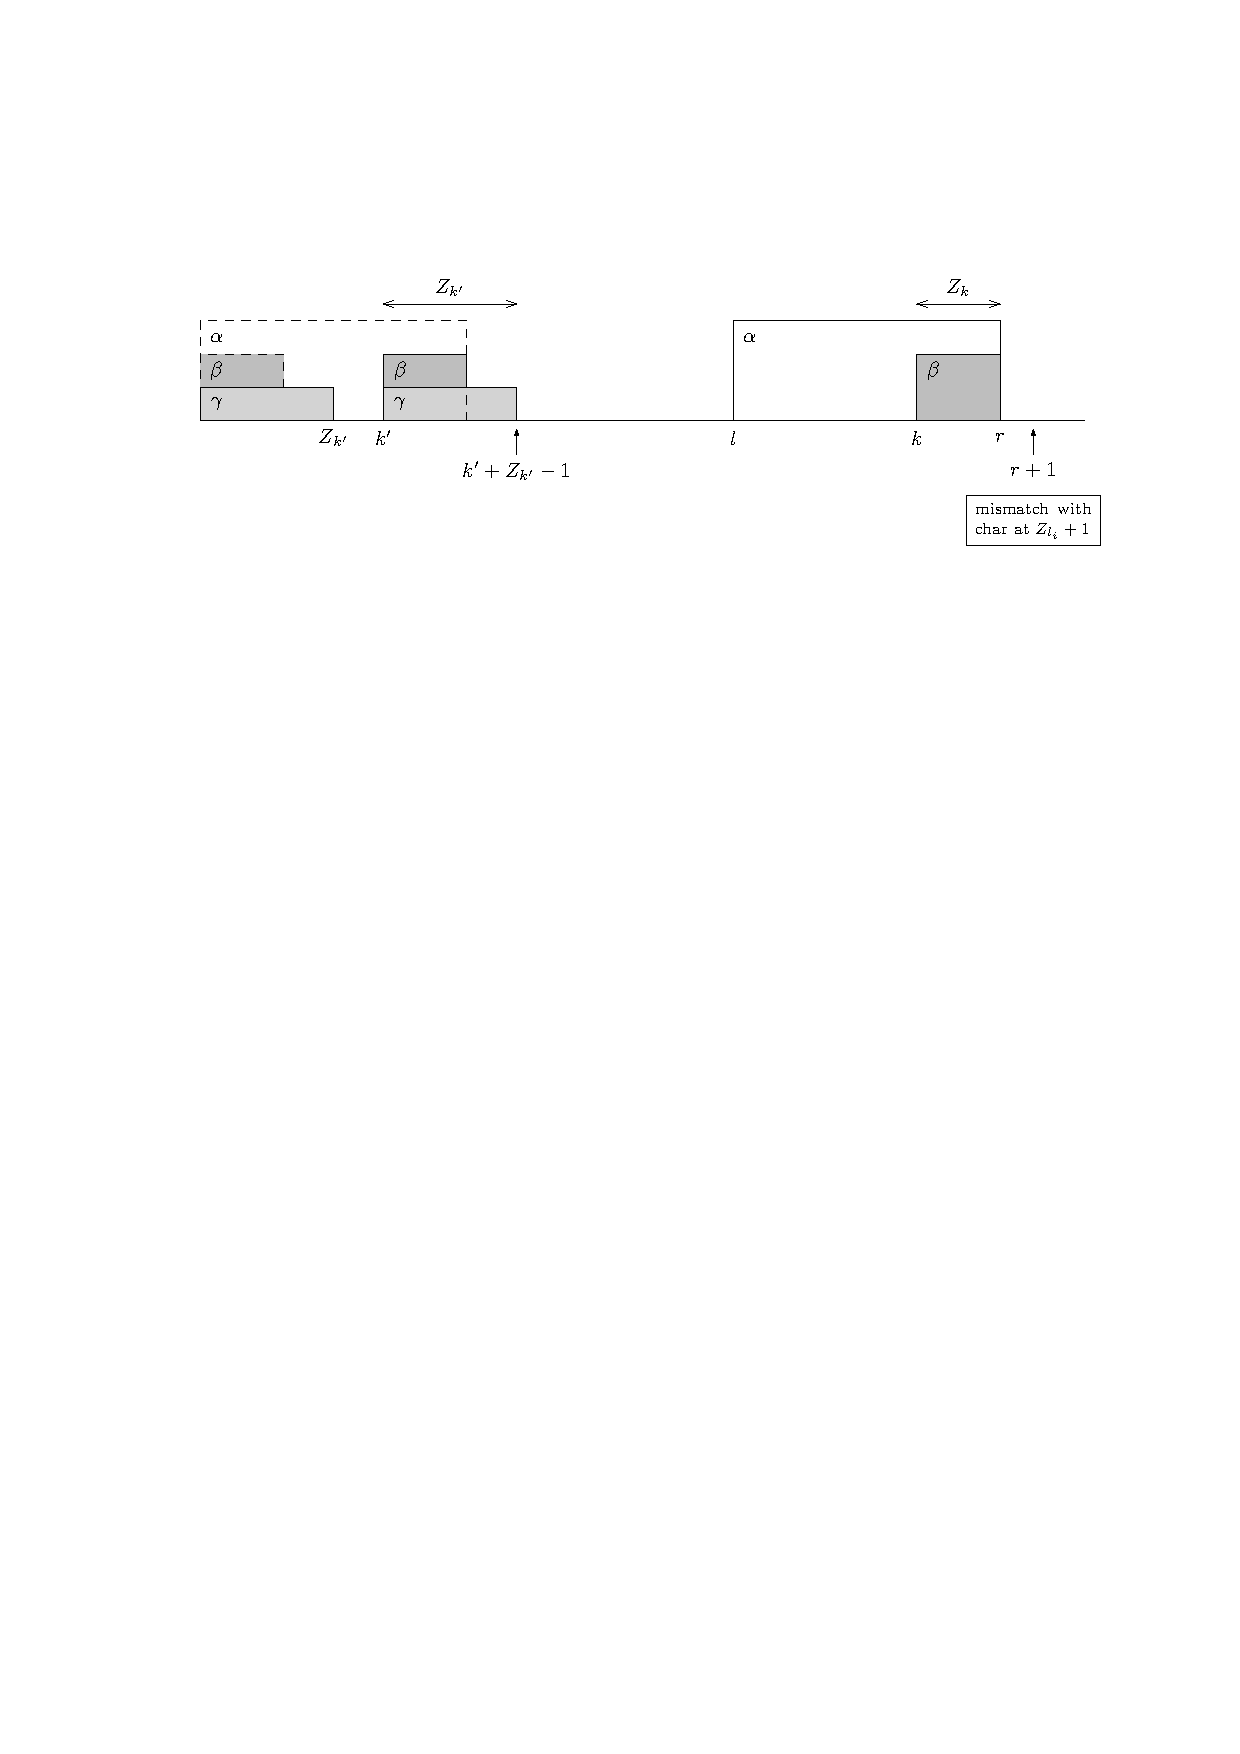
\includegraphics[width=\linewidth]{z/z-process-case2b1.pdf}
    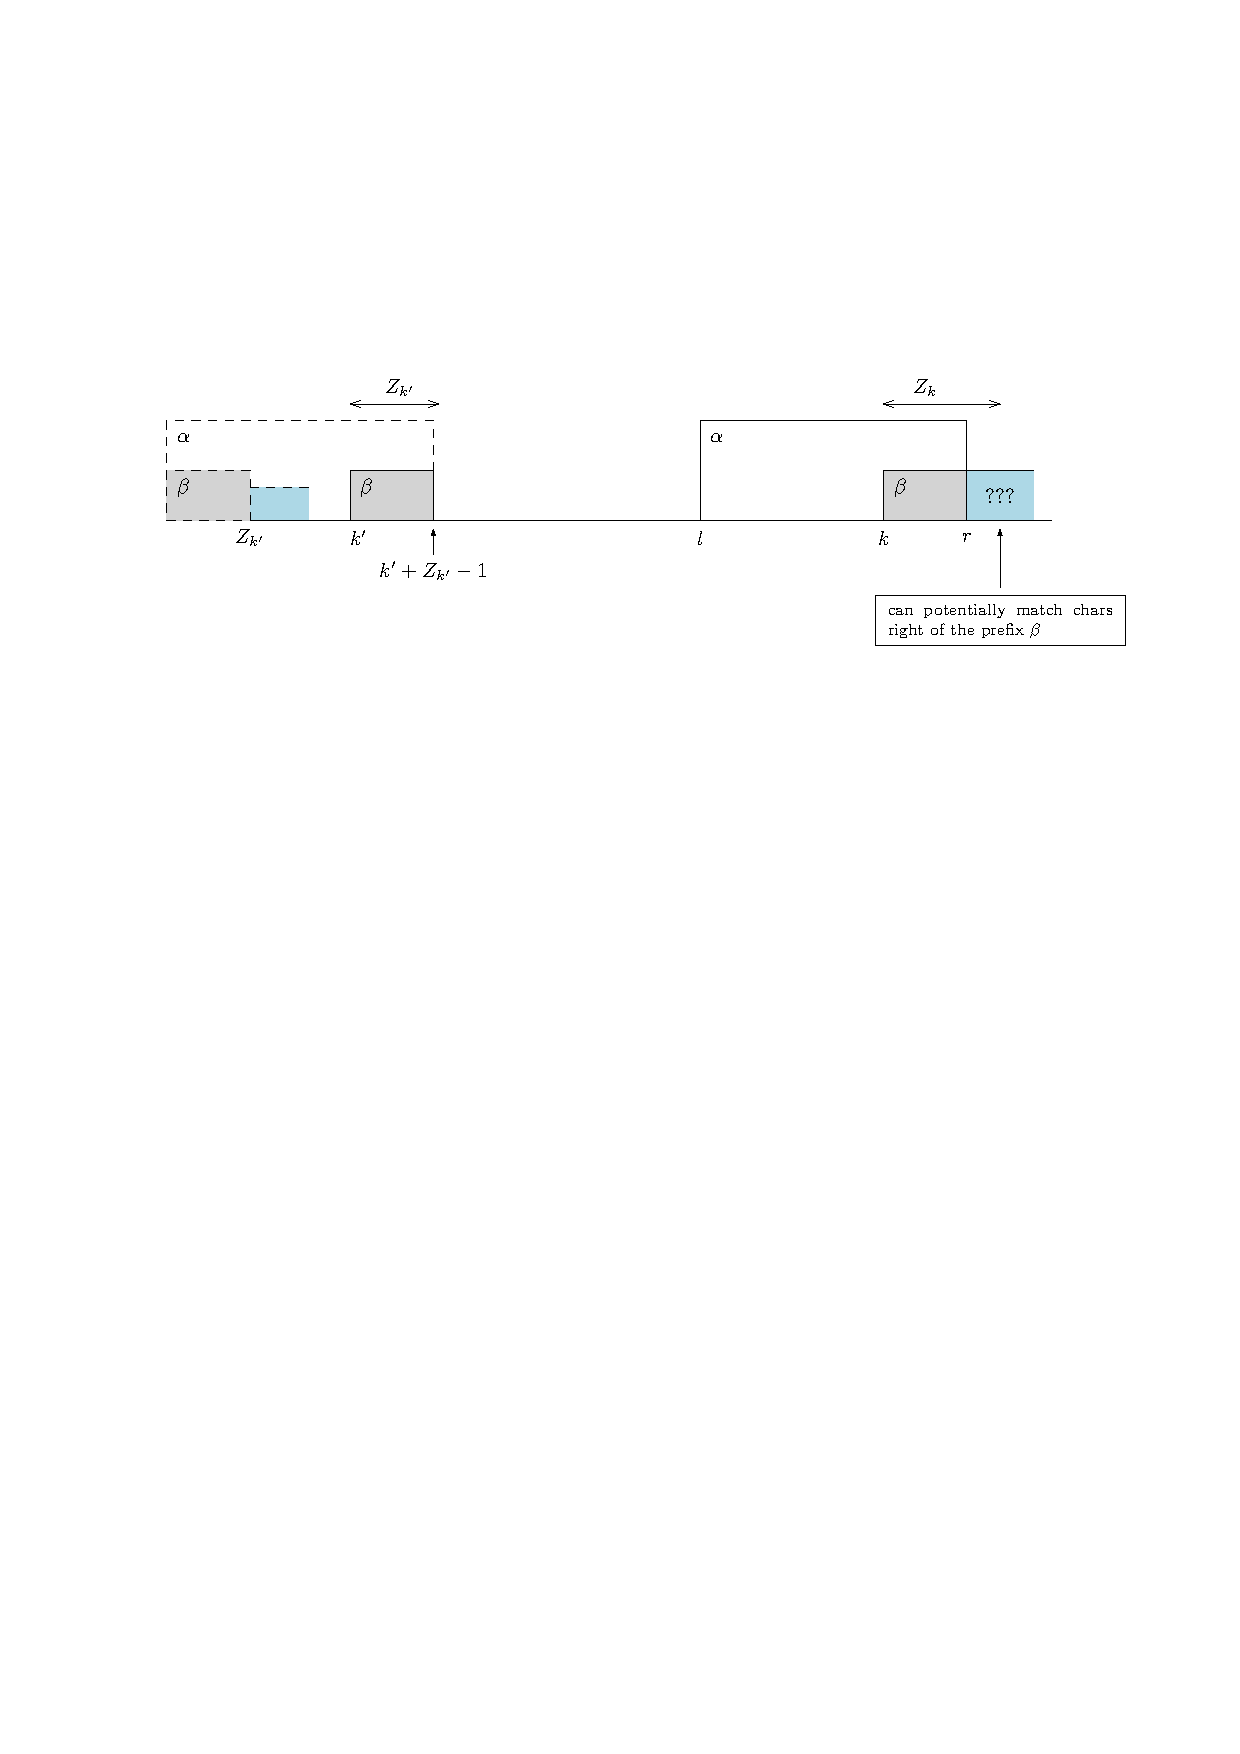
\includegraphics[width=\linewidth]{z/z-process-case2b2.pdf}
    \caption{Case 2b: The longest string starting at $k'$ that matches a prefix of $S$ is at least $|\beta| = r-k+1$. In this case, we continue to compare characters right of $r$ with characters right of the $Z_{k'}$th character until mismatch. }
    \label{fig:z-process-case2b}
\end{figure}

Given $Z_i$ for all $1 < i \leq k-1$ and the current $l$ and $r$, we can compute $Z_k$ using the following procedure:

\begin{enumerate}
    \item Case 1: If $k > r$, $k$ is not in an existing Z-box. Compute $Z_k$ by explicitly comparing each character starting at $k$ with prefix of $S$.
    \item Case 2: If $k \leq r$, $k$ is in an existing Z-box, denoted $\alpha$, that matches a prefix of $S$. Hence, character $S[k]$ also appears in the prefix at position $k' = k - l + 1$. \\ We also consider the substring $S[k\ldots r]$, denoted $\beta$. By the same reasoning, $\beta$ matches the substring $S[k'\ldots Z_l]$.
    \begin{enumerate}
        \item $Z_{k'} < |\beta|$. This implies that the longest string starting at $k'$ that matches a prefix of $S$, $\gamma$, is shorter $|\beta|$. Then, $Z_{k} = Z_{k'}$, and $l,r$ remain unchanged. Note that $|\gamma|$ can be 0.
        \item $Z_{k'} \geq |\beta|$. This means $S[k\ldots r]$ is at least a prefix of $S$. However, $Z_k$ might be larger than $|\beta|$. We cannot determine this solely based on the existing information as characters beyond the $Z_l$th character are not included in $\alpha$. So, we compare the characters starting at position $r+1$ of $S$ to the characters starting at position $|\beta|+1$ of $S$, until a mismatch occurs. Say the mismatch occur at position $q$. Then, $Z_k = q- k$, $r = q-1$, and $l = k$. (If $Z_{k'} > |\beta|$, a mismatch occurs immediate after the $Z_{l}$th character because otherwise, the $(r+1)$th character matches the $Z_{l}$th character, and we would have a longer $\alpha$ and a larger $Z_l$)
    \end{enumerate}
\end{enumerate}

\begin{codebox}
    \Procname{$\proc{Compute-Z}(S)$}
    \li $n = |S|$
    \li $l,r,k = 1$
    \li $Z = \text{empty array of length $n$}$
    \li \For $k=2$ \To $n$ \Do
        \li \If $k > r$ \Then \RComment{Case 1}
            \li \Comment{compute $Z[k]$ from scratch}
            \li $l,r = k$ 
            \li \While $r \leq n$ \textbf{and} $S[r-l+1] \isequal S[r]$ \Do
                \li $r = r + 1$
            \End
            \li $Z[k] = r-l$
            \li $r = r - 1$
        \li \Else \RComment{Case 2}
            \li $k' = k - l + 1$
            \li \If $Z[k'] < r - k + 1$ \Then \RComment{Case 2a}
                \li $Z[k] = Z[k']$ 
            \li \Else \RComment{Case 2b}
                \li $q = r+1$
                \li \While $q \leq n$ \textbf{and} $S[q-l + 1] \isequal S[q]$ \Do
                    \li $q = q + 1$
                \End
                \li $Z[k] = q-k$
                \li $l,r = k, \,q-1$ 
            \End
        \End
        \End
        \li \Return $Z$ 
\end{codebox}

For a step-by-step animation of the Z algorithm, see \\
\href{https://personal.utdallas.edu/~besp/demo/John2010/z-algorithm.htm}{https://personal.utdallas.edu/\textasciitilde besp/demo/John2010/z-algorithm.htm}

\section{Running Time of the Z Algorithm}

\begin{theorem}
    All the $Z_i$ values can be computed by the Z algorithm with at most $2|S| \in O(|S|)$ comparisons.
\end{theorem}

\begin{proof}
    The time is proportional to the number of iterations, $|S|$, plus the number of character comparisons.
    
    Each iteration that does any character comparison ends as soon as there is a mismatch, so there are at most $|S|$ \textbf{mismatches}. In every iteration where there is a match, $r$ moves to the right by an amount at least as large as the number of matches. This implies that there are at most $|S|$ \textbf{matches}. Note that once a character results in a match, it is not compared again.

    Every character comparison is either a match or mismatch, so the total number of comparisons is at most $2|S|$.
\end{proof}

\section{Correctness of the Z Algorithm}

\begin{theorem}
    At the $k$th iteration of the algorithm, \proc{Compute-Z} correctly calculates $Z_k$, and $l,r$ are updated correctly.
\end{theorem}

\begin{proof}
    By a case analysis.

    Case 1: Trivial since it's just explicit comparison.

    Case 2a: We claim that the substring at position $k$ can match a prefix of $S$ only for length $Z_{k'} < |\beta|$. Prove the claim by contradiction (suppose not, we would have a longer prefix matching the substring at $k'$, contradicting the maximality of $Z_{k'}$).

    Case 2b: $\beta$ must be a prefix of $S$ as established above. Characters beyond $r$ are explicitly compared.
\end{proof}

\begin{corollary}
    \proc{Compute-Z} correctly calculates $Z_k$ for all $k \in \{2,\ldots,|S|\}$.
\end{corollary}

\begin{proof}
    By induction on $k$.
\end{proof}

\section{Z Algorithm for Exact Matching}

The Z algorithm lends itself to a linear-time algorithm for exact matching. Given a pattern $P$ and text $T$, we construct a new string $P \$ T$ where $\$$ is a \textit{\textbf{separator}} (a.k.a. \textit{\textbf{delimiter}} or \textit{\textbf{sentinel}}) such that $\$ \not\in \Sigma$. We construct the Z-array for this new string. It takes $O(|P|+|T|)$ time to construct the Z-array. After this, we can simply make a pass through the Z-array and read the result from it. This takes $O(|T|)$ time.

\begin{codebox}
    \Procname{$\proc{Z-Exact-Matching}(P,T)$}
    \li $\id{query} = P + ``\$" + T$
    \li $Z = \proc{Compute-Z}(\id{query})$
    \li \For $i = |P|+1$ \To $|P|+|T|+1$ \Do
        \li \If $Z[i] \isequal |P|$ \Then
            \li pattern found at index $i - |P|$ 
\end{codebox}

\chapter{Boyer-Moore}

\chapter{Knuth-Morris-Pratt Algorithm}

\backmatter

\bibliography{sample-handout}
\bibliographystyle{plainnat}


\printindex

\end{document}

